\documentclass[10pt,]{beamer}
\usepackage{beamerthemeblackboard}
\usepackage{graphics}
\usepackage{emerald}
\usepackage[T1]{fontenc}

%\usepackage{emerald}
\usefonttheme{professionalfonts} % using non standard fonts for beamer
\usefonttheme{serif} % default family is serif
\usepackage{fontspec}
%\usefonttheme{serif}     % Font theme: serif
%\usepackage{ccfonts}     % Font family: Concrete Math
%\usepackage[T1]{fontenc} % Font encoding: T1


%\usepackage{eulervm}
\title{Robust Support Vector Machines for Classification}
%\author{J. Watson} 
%\institute{\small{Baker St Publications}}
%\date{{10 September 2016}}

\author[statistics]{I. Vranckx, J. Schreurs, B. De Ketelaere, M. Hubert and J.Suykens}
%\cortext[mycorrespondingauthor]{Corresponding author}
%\ead[url]{wis.kuleuven.be/stat/robust}
%\ead[mail]{iwein.vranckx@kuleuven.be}

%\author[stadius]{Joachim Schreurs}
%\author[mebios]{Bart De Ketelaere}
%\author[statistics]{Mia Hubert}
%\author[stadius]{Johan Suykens}
%
%\address[statistics]{KU Leuven, Department of Mathematics and LStat, Celestijnenlaan 200B, BE-3001 Heverlee, Belgium}
%\address[stadius]{KU Leuven, ESAT-STADIUS, Kasteelpark Arenberg 10, BE-3001 Heverlee, Belgium}
%\address[mebios]{KU Leuven, Division of Mechatronics, Biostatistics and Sensors, Kasteelpark Arenberg 30, BE-3001 Heverlee, Belgium}

\begin{document}

%set the font to Augie (emerald font).
%Comment out this line to only use Augie
%for titles, etc
\ECFAugie

%title frame
\begin{frame}[plain]
\maketitle  
\end{frame}

\begin{frame}{Overview}
In this talk I will talk about joint work with: ...
\end{frame}


\begin{frame}{Kernel feature space}
As a warm-up, we'll introduce the kernel feature space by an example.
\end{frame}

\begin{frame}{Linear Regression}
Define a \textit{linear} regression problem, given a
dataset $ \{x_{i},y_{i}\}_{i=1}^{^{n}}\in \mathbb{R}$ as follows:
\begin{equation}
	y_{i}=w^{T}x_{i}+\epsilon_{i}
	\label{eq:regression}
\end{equation}

Here $\epsilon_{i}$ is assumed to be white noise. Least squares is used to obtain an estimate $\hat{w}$ of $w$. \\
\vspace{0.5cm}
If the system from which the data are collected is linear, the
regression provides a good approximation of the system behaviour. 
\end{frame}

\begin{frame}
However, if the true system follows the non-linear process:
\begin{equation}
y=w_{1}x^{2}+w_{2}\sqrt{2}x_{i}+w_{3}+\epsilon_{i}
\end{equation}
The regression is not correctly specified because it does not contain
the non-linear effect $x^{2}$. \\
\vspace{0.5cm}
To obtain the correct specification, the original input $x$ can be mapped to a higher dimensional space
by means of the feature map $\varphi:\mathbb{R}\rightarrow\mathbb{R}^{3}$, in this example defined by:
\begin{equation}
\varphi(x)=[x^{2},\sqrt{2}x,1]
\end{equation}
\end{frame}

\begin{frame}
Solving the regression
\begin{equation}
y_{i}=w^{T}\varphi(x_{i})+\epsilon_{i}
\end{equation}

...yields an estimate of $w=[w_1,w_2,w_3]$. In this example, the feature
map $\varphi(x)$ is assumed to be known, and thus the coordinates
in the high-dimensional space can be computed directly to arrive at
the correct regression specification. 
\end{frame}

\begin{frame}
However, note that a feature map $\varphi(x)$ does not have to be known explicitly: non-linear
transformations are rather implicitly defined by kernel functions.  \\
\vspace{0.5cm}
For example, the inner product of two vectors is defined as:
\begin{eqnarray}
\varphi(x_{1})^{T}\varphi(x_{2}) & = & [x_{1}^{2},\sqrt{2}x_{1},1]^{T}.[x_{2}^{2},\sqrt{2}x_{2},1]\\
%& = & x_{1}^{2}x_{2}^{2}+2x_{1}x_{2}+1\\
%& = & (x_1 x_2+1)^{2}
\end{eqnarray}

Which is equivalent to following kernel function:
\begin{equation}
K(x_{1},x_{2})=(x_{1}^{T}x_{2}+1)^{d}\qquad d\,\in\mathbb{I}
\label{eq:polykernel}
\end{equation}
\end{frame}


\begin{frame}
Assuming $x_1$ and $x_2$ are two input samples in the original $\mathbb{R}^p$ space and they are
mapped into the feature space as $\varphi(x_1)$ and $\varphi(x_2)$, the inner product in the feature space has an equivalent kernel in the original input space, i.e. 

\begin{equation}
	\varphi(x_1)^T \varphi(x_2)=K(x_1,x_2)
\end{equation}

This is called the kernel trick, where $K(.,.)$ is a
positive definite function that satisfies Mercer's conditions. Plugging this equation into the regression formula \ref{eq:regression} yields its 'kernelized' form, in  this example effectively acting in $\mathbb{R}^3$ space. 
\end{frame}

\begin{frame}
The following principle illustrates this feature transformation principle graphically. 
	\begin{figure}
		\centering
		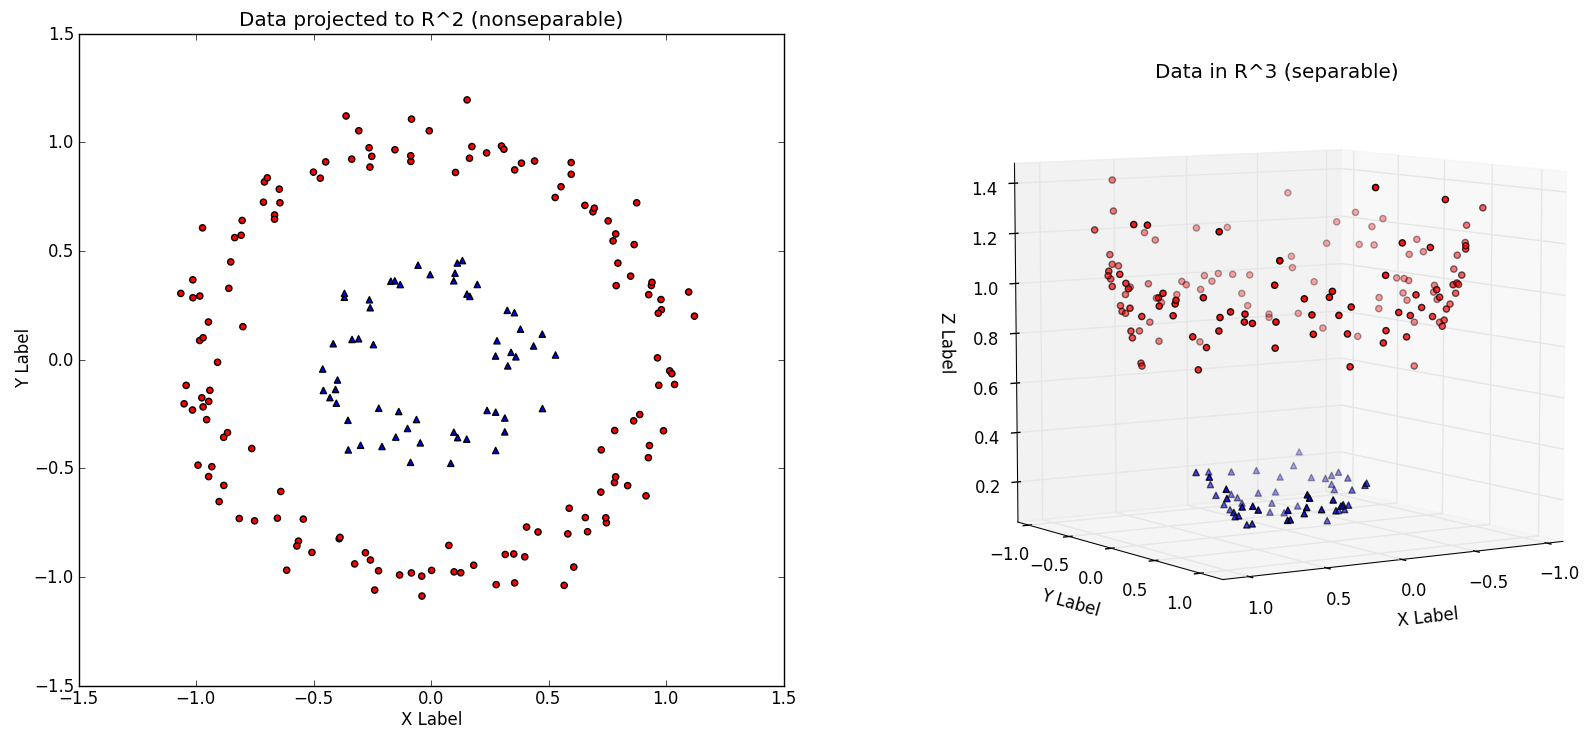
\includegraphics[width=0.9\linewidth]{twocirles}
		\label{fig:twocirles}
	\end{figure}
	
\end{frame}


\begin{frame}{Take away message}
In a nutshell, kernel transformations allows us to construct non-linear, high potential classifiers.  At the same time, the accurate working of the used optimization routine (and all other algorithms involved) becomes increasingly important.
\end{frame}

\begin{frame}{}
	\huge Robust Support Vector Machines
\end{frame}

\end{document}
